

\subsection{Princípio da Inversão de Dependência (Dependency Inversion Principle - DIP)}
    
    \par O DIP estabelece que módulos de alto nível não devem depender de módulos de baixo nível; ambos devem depender de abstrações. Adicionalmente, as abstrações não devem depender de detalhes concretos, mas sim os detalhes é que devem depender das abstrações. Isso significa que as classes que contêm a lógica de negócios principal (alto nível) não devem ser diretamente acopladas a classes que lidam com detalhes de infraestrutura (baixo nível) \cite{livro:martin:cleanarch}.

    \par Este princípio é crucial para criar sistemas desacoplados e flexíveis, pois promove a dependência de interfaces ou classes abstratas em vez de implementações concretas. Isso permite que as implementações de baixo nível possam ser alteradas ou substituídas sem impactar os módulos de alto nível, desde que o contrato definido pela abstração seja mantido. Tal desacoplamento também facilita os testes, permitindo a substituição de dependências reais por dublês de teste \cite{livro:joshi:2016}.

    \par A Figura~\ref{fig:figura_dip_bad} mostra um exemplo de violação do DIP.

    \begin{figure}[H]
        \centering
        
        \caption{Violação da DIP.}
        \label{fig:figura_dip_bad} 
        
        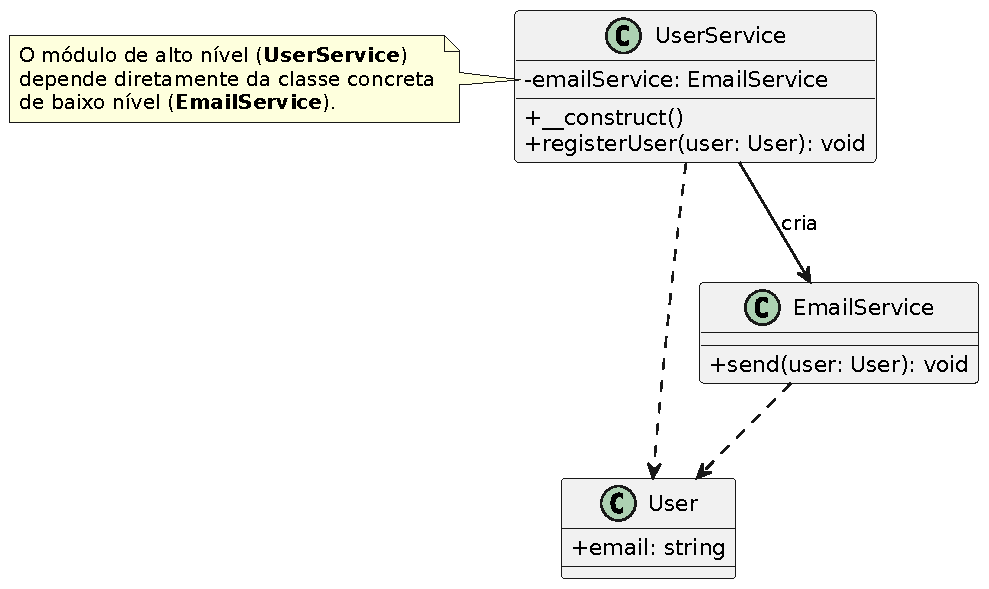
\includegraphics[width=1\linewidth]{figuras/solid/dip_bad.pdf}
 
        \fonte{Adaptado de \cite{artigo:ramachandrappa:2024}.}
    \end{figure}

    \par Nesse exemplo, nota-se uma classe UserService (alto nível) que depende diretamente de uma classe concreta EmailService (baixo nível) está fortemente acoplada. Esse problema é resolvido na Figura \ref{fig:figura_dip_good}.

    \begin{figure}[H]
        \centering   
        
        \caption{Aplicação da DIP.}
        \label{fig:figura_dip_good}
        
        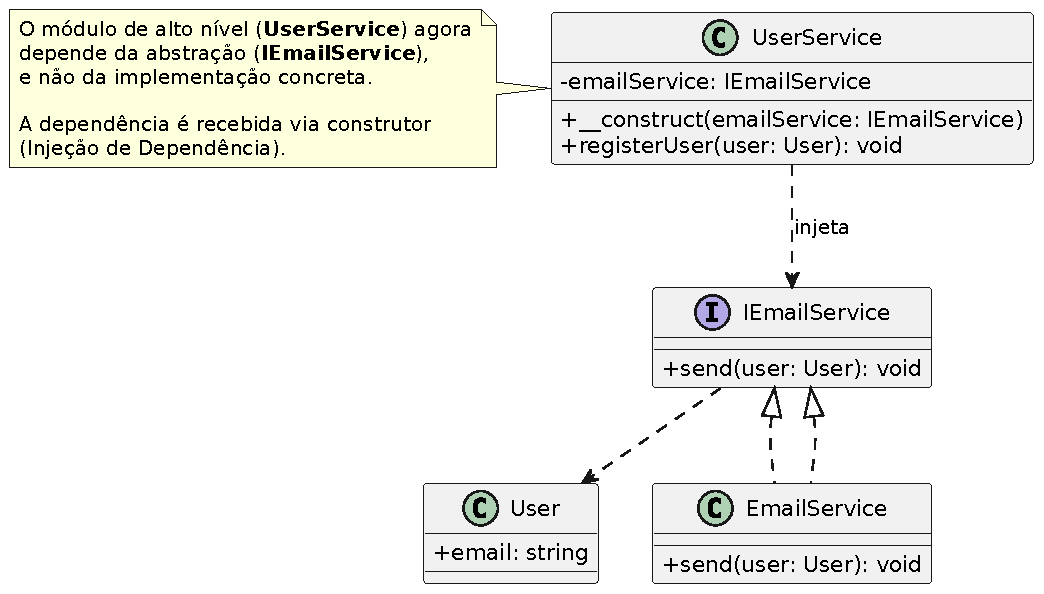
\includegraphics[width=1\linewidth]{figuras/solid/dip_good.pdf}

        
        \fonte{Adaptado de \cite{artigo:ramachandrappa:2024}.}
    \end{figure}
    
    \par Essa solução da Figura \ref{fig:figura_dip_good}, mostra a criação da interface IEmailService, onde UserService depende dessa interface e EmailService implementa IEmailService. Isso inverte a direção da dependência, conforme o DIP prega, agora o UserService não depende do detalhe mas sim da abstração \cite{artigo:ramachandrappa:2024}.